% =============================================================
%  Extra Study #001 — English by Jay
%  "The English words you don't learn unless you go to England."
%  Companion sheet: read alongside the video
% =============================================================
\documentclass[11pt,a4paper]{article}
\usepackage[T1]{fontenc}
\usepackage[utf8]{inputenc}
\usepackage[scaled]{helvet}
\renewcommand{\familydefault}{\sfdefault}
\usepackage{tipa}
\usepackage{amssymb}
\usepackage[margin=2cm,top=1.6cm]{geometry}
\usepackage{xcolor}
\usepackage{tikz}
\usepackage{graphicx}
\usetikzlibrary{shapes,positioning,calc,decorations.pathmorphing}
\usepackage[most]{tcolorbox}
\usepackage{enumitem}
\usepackage{multicol}
\usepackage{tabularx}
\usepackage{array}
\usepackage{fancyhdr}
\usepackage[hidelinks]{hyperref}

% ---------- Sprout-inspired palette ----------
\definecolor{sprout}{HTML}{2E9E5B}
\definecolor{sproutdark}{HTML}{1D6B3C}
\definecolor{sproutlight}{HTML}{E8F6EE}
\definecolor{tea}{HTML}{B5722F}
\definecolor{tealight}{HTML}{FBF1E6}
\definecolor{ink}{HTML}{22313F}
\definecolor{sky}{HTML}{2F6FB5}
\definecolor{skylight}{HTML}{EAF2FB}
\definecolor{coral}{HTML}{D9534F}
\definecolor{corallight}{HTML}{FDEDEC}
\color{ink}

\setlength{\parindent}{0pt}
\setlength{\parskip}{4pt}
\setlist{nosep,leftmargin=1.4em}

\pagestyle{fancy}
\fancyhf{}
\renewcommand{\headrulewidth}{0pt}
\fancyfoot[L]{\footnotesize\color{sproutdark}Extra Study \#001 · English by Jay}
\fancyfoot[R]{\footnotesize\color{sproutdark}\thepage}

% ---------- little sprout logo ----------
\newcommand{\sproutlogo}[1][1]{%
\begin{tikzpicture}[scale=#1,baseline=-0.5ex]
  \draw[sproutdark,line width=1.2pt] (0,-0.35) -- (0,0.05);
  \fill[sprout] (0,0.05) .. controls (-0.35,0.05) and (-0.45,0.35) .. (-0.45,0.4) .. controls (-0.2,0.42) and (0,0.3) .. (0,0.05);
  \fill[sprout!70] (0,0.05) .. controls (0.3,0.1) and (0.4,0.45) .. (0.4,0.5) .. controls (0.15,0.5) and (0,0.35) .. (0,0.05);
\end{tikzpicture}}

% ---------- boxes ----------
\newtcolorbox{wordcard}[3]{enhanced,breakable,colback=white,colframe=sprout,
  boxrule=1pt,arc=3mm,left=3mm,right=3mm,top=2mm,bottom=2mm,
  fonttitle=\bfseries\large,coltitle=white,colbacktitle=sprout,
  title={\sproutlogo[0.55]\hspace{2mm}#1\quad{\normalsize\textnormal{\let\ipa\ipatitle #2}}},
  attach boxed title to top left={yshift=-2mm,xshift=3mm},
  boxed title style={arc=2mm,boxrule=0pt},before skip=8pt,after skip=6pt}

\newtcolorbox{tipbox}[1][Jay's tip]{enhanced,colback=tealight,colframe=tea,boxrule=0.6pt,
  arc=2mm,left=2mm,right=2mm,top=1mm,bottom=1mm,
  title={\bfseries #1},fonttitle=\small,coltitle=tea,colbacktitle=tealight,
  attach title to upper={\ \ },before skip=4pt,after skip=4pt}

\newtcolorbox{infobox}[1]{enhanced,breakable,colback=skylight,colframe=sky,boxrule=0.8pt,arc=2mm,
  title={\bfseries #1},coltitle=white,colbacktitle=sky,left=3mm,right=3mm}

\newtcolorbox{warnbox}[1]{enhanced,colback=corallight,colframe=coral,boxrule=0.8pt,arc=2mm,
  title={\bfseries #1},coltitle=white,colbacktitle=coral,left=3mm,right=3mm}

\newtcolorbox{exbox}[2][breakable]{enhanced,#1,colback=sproutlight,colframe=sproutdark,
  boxrule=0.8pt,arc=2mm,title={\bfseries #2},coltitle=white,colbacktitle=sproutdark,
  left=3mm,right=3mm,before skip=8pt}

% heard-it checkbox + timestamp line
\newcommand{\heard}{\unskip\nobreak\hfill\mbox{\small\color{sproutdark}$\square$ heard it at \underline{\hspace{1.4cm}}}}
\newcommand{\ipa}[1]{{\color{sproutdark}\textipa{#1}}}
\newcommand{\ipatitle}[1]{{\color{white}\textipa{#1}}}
\newcommand{\blank}[1][2.6cm]{\underline{\hspace{#1}}}
\newcommand{\ex}[1]{\textit{\color{ink!80}``#1''}}

\begin{document}

% =================== HEADER ===================
\begin{tikzpicture}[remember picture,overlay]
  \fill[sprout] (current page.north west) rectangle ($(current page.north east)+(0,-3.1cm)$);
  \fill[sproutdark] ($(current page.north west)+(0,-3.1cm)$) rectangle ($(current page.north east)+(0,-3.3cm)$);
  \node[anchor=north west,text=white,font=\bfseries\small] at ($(current page.north west)+(2cm,-0.6cm)$) {EXTRA STUDY \#001 \quad·\quad English by Jay \quad·\quad B1 \quad·\quad $\approx$ 11 min};
  \node[anchor=north west,text=white,font=\bfseries\LARGE,text width=14cm] at ($(current page.north west)+(2cm,-1.15cm)$) {The English words you don't learn unless you go to England.};
  \node at ($(current page.north east)+(-2.2cm,-1.6cm)$) {\sproutlogo[2.6]};
\end{tikzpicture}
\vspace*{2.0cm}

\begin{multicols}{2}
\textbf{\color{sproutdark}Watch:} \href{https://www.youtube.com/watch?v=IXuJSwk1gck}{\color{sky}\underline{youtube.com/watch?v=IXuJSwk1gck}}\\
\textbf{\color{sproutdark}What it covers:} 7 everyday British words and phrases that most textbooks skip, a few pronunciation habits (dropped T's, the glottal stop) and a hidden ``secret word''.

\columnbreak
\textbf{\color{sproutdark}How to use this sheet}
\begin{enumerate}
  \item Do \textbf{Warm-up} before you press play.
  \item Keep the \textbf{word cards} open while you watch. Tick each one and write the timestamp when Jay says it.
  \item Do the \textbf{exercises} afterwards. The answer key is on the last page.
\end{enumerate}
\end{multicols}

\begin{warnbox}{A note on the order}
I couldn't open the video's captions, so I can't promise the cards below follow Jay's exact order. They follow the order of the video's description, and the facts come from the description, the video's vocabulary list (VoiceTube) and standard British usage. If Jay's order is different, just use the timestamp boxes, and keep an eye out for an 8th word, the ``secret word''.
\end{warnbox}

% =================== WARM-UP ===================
\begin{exbox}{\sproutlogo[0.5]\ Warm-up · before you watch (2 min)}
\begin{enumerate}
  \item Have you heard any of these from British players online? \textbf{cheers · innit · gutted · proper · cheeky}. Guess what each one means.
  \item \textbf{Prediction:} Jay calls them words ``you don't learn unless you go to England''. Why might a textbook leave them out?
  \item Say \ex{a cup of tea} quickly, five times. What happens to the word \textit{of}?
\end{enumerate}
\end{exbox}

% =================== WORD CARDS ===================
\section*{\color{sproutdark}\sproutlogo[0.8]\ The words}

% ---- 1 cuppa ----
\begin{wordcard}{1 · cuppa}{\ipa{/"k2p@/} \quad noun, informal}{}
\begin{minipage}[t]{0.66\linewidth}\vspace{0pt}
\textbf{Meaning:} a cup of tea (sometimes coffee).\heard\\[2pt]
\ex{Fancy a cuppa?} = Would you like a cup of tea?\\
\ex{I'll put the kettle on and make us a cuppa.}

\textbf{Why it sounds like that:} \textit{cup of} \(\rightarrow\) \textit{cup'a}. The weak form of \textit{of} is just \ipa{/@/}, and in fast speech the /v/ disappears.

\textbf{Family words to listen for:} \textbf{brew} (\ex{Shall I make a brew?}, mainly northern England), \textbf{kettle}, \textbf{mug}, \textbf{biscuit}, \textbf{to dunk} (dip a biscuit in your tea), \textbf{digestive} (a plain British biscuit), \textbf{fancy} (= want).
\end{minipage}\hfill
\begin{minipage}[t]{0.31\linewidth}\vspace{0pt}\centering
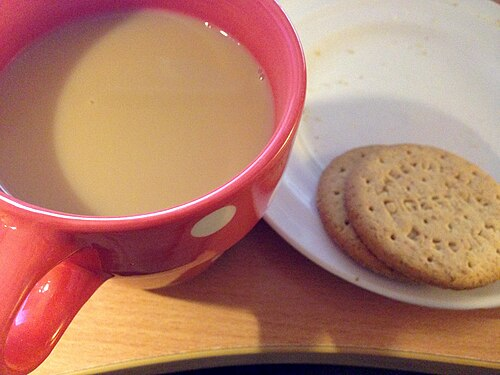
\includegraphics[width=\linewidth]{img/tea.jpg}\\[-1pt]
{\scriptsize\color{tea}a cuppa and two digestives\\(ready for dunking)}
\end{minipage}
\begin{tipbox}
The description spells it ``cupper'', but the normal spelling is \textbf{cuppa}. A \textbf{proper cuppa} is a real, strong cup of tea, made properly (see card 7).
\end{tipbox}
\end{wordcard}

% ---- 2 cheeky ----
\begin{wordcard}{2 · cheeky}{\ipa{/"tSi:ki/} \quad adjective}{}
\textbf{Meaning 1:} slightly rude or disrespectful, but in a playful or funny way.\heard\\
\ex{Don't be cheeky!} \quad \ex{He gave me a cheeky grin.}

\textbf{Meaning 2 (very British):} used for a small treat or something done on impulse, a bit naughty but harmless.\\
\ex{Fancy a cheeky biscuit?} \quad \ex{Let's get a cheeky pint after the lab.}

\begin{tipbox}[In your games]
\ex{That was a cheeky flank!} means a sneaky, slightly unfair but clever play. Usually it's a compliment, not an insult.
\end{tipbox}
\end{wordcard}

% ---- 3 gutted ----
\begin{wordcard}{3 · gutted}{\ipa{/"g2PId/} \quad adjective, informal}{}
\begin{minipage}[t]{0.70\linewidth}\vspace{0pt}
\textbf{Meaning:} extremely disappointed or sad about something.\heard\\
\ex{I'm gutted we lost on the last point.}\\
\ex{She was absolutely gutted when the concert was cancelled.}

\textbf{Sound:} the \textit{tt} often becomes a \textbf{glottal stop} \ipa{/P/}, so it sounds like ``gu'-id''. Listen for it!

\textbf{Strong words go together:} \textit{absolutely gutted}, \textit{proper gutted}, \textit{devastated} (even stronger).
\end{minipage}\hfill
\begin{minipage}[t]{0.26\linewidth}\vspace{0pt}\centering

\includegraphics[width=2.0cm]{img/gutted.png}\\[-2pt]
{\scriptsize\bfseries\color{sky}gutted}
\end{minipage}
\end{wordcard}

% ---- 4 buzzing ----
\begin{wordcard}{4 · buzzing}{\ipa{/"b2zIN/} \quad adjective, informal}{}
\begin{minipage}[t]{0.70\linewidth}\vspace{0pt}
\textbf{Meaning:} very excited, happy or full of energy.\heard\\
\ex{I'm buzzing for the new season!}\\
\ex{The whole team was buzzing after the win.}

\textbf{Opposite pair:} \textit{gutted} \(\leftrightarrow\) \textit{buzzing}. A perfect pair for after a match.

\textbf{Also:} \textit{The place was buzzing} = full of people and activity. (A \textbf{buzz} is the sound bees make.)
\end{minipage}\hfill
\begin{minipage}[t]{0.26\linewidth}\vspace{0pt}\centering

\includegraphics[width=2.0cm]{img/buzzing.png}\\[-2pt]
{\scriptsize\bfseries\color{sproutdark}buzzing}
\end{minipage}
\end{wordcard}

% ---- 5 innit ----
\begin{wordcard}{5 · innit}{\ipa{/"InIP/} \quad question tag, very informal}{}
\textbf{Meaning:} a short form of \textit{isn't it}, used to ask for agreement or just to keep the conversation going.\heard\\
\ex{It's freezing today, innit?} = It's freezing, isn't it?

\textbf{The surprising part:} in casual London speech, \textit{innit} can follow \emph{any} subject or tense:\\
\ex{You're from Belgium, innit?} (= aren't you?) \quad \ex{He played well, innit?} (= didn't he?)

\begin{tipbox}[Grammar link]
Standard English changes the tag to match the verb: \textit{It \textbf{is}\ldots{} isn't it? · You \textbf{are}\ldots{} aren't you? · He \textbf{played}\ldots{} didn't he?} \textit{Innit} skips all of that. Understand it, but in exams always use the full, matching tag.
\end{tipbox}
\end{wordcard}

% ---- 6 cheers ----
\begin{wordcard}{6 · cheers}{\ipa{/tSI@z/} \quad exclamation}{}
\textbf{Three uses:}\heard
\begin{enumerate}
  \item \textbf{Thank you} (the most common): \ex{Cheers, mate!} when someone passes you the salt, or revives you in a game.
  \item \textbf{Goodbye}: \ex{Right, cheers then, see you tomorrow.}
  \item \textbf{A toast} when you lift your glasses together: \ex{Cheers!}
\end{enumerate}
\textbf{Sound:} no /r/! Southern British English is \textbf{non-rhotic}, so \textit{cheers} sounds like ``chee-uhz''.
\end{wordcard}

% ---- 7 proper ----
\begin{wordcard}{7 · proper}{\ipa{/"pr6p@/} \quad adjective / adverb, informal}{}
\textbf{Meaning 1 (adj.):} real, genuine, done correctly.\heard\\
\ex{Let's have a proper cup of tea.} \quad \ex{We need a proper plan this time.}

\textbf{Meaning 2 (adv., informal):} very, really.\\
\ex{That boss fight was proper hard.} \quad \ex{I'm proper tired.}

\textbf{Sound:} again the final \textit{-er} is just \ipa{/@/}, with no /r/.
\end{wordcard}

% ---- secret ----
\begin{wordcard}{8 · the secret word}{\textit{your turn}}{}
Jay hides an extra word somewhere in the video. When you hear it, write it here:\\[4pt]
Word: \blank[4cm] \quad Meaning: \blank[6cm] \quad Time: \blank[1.4cm]
\end{wordcard}

% =================== PRONUNCIATION LAB ===================
\section*{\color{sproutdark}\sproutlogo[0.8]\ Pronunciation lab: why British speech is hard to catch}

\begin{minipage}[t]{0.52\linewidth}\vspace{0pt}
\textbf{1. The glottal stop \ipa{/P/}.} Many British speakers replace a /t/ in the middle or at the end of a word with a tiny ``catch'' in the throat: the vocal folds snap shut for a moment, like in the middle of \textit{uh-oh}.

\begin{tabularx}{\linewidth}{>{\bfseries}l X}
better & ``be'-uh'' \ipa{/"beP@/}\\
water & ``wa'-uh'' \ipa{/"wO:P@/}\\
a lot of & ``a lo' of'' \ipa{/@"l6P@v/}\\
gutted & ``gu'-id''\\
innit & ``inni''' \\
\end{tabularx}

\textbf{2. No /r/ after vowels} (non-rhotic): \textit{cheers, proper, better, here} have no /r/ sound unless the next word starts with a vowel (\textit{better \textbf{r}off}).

\textbf{3. Weak forms:} \textit{of, to, for, a} shrink to \ipa{/@/}: \textit{cup of} \(\rightarrow\) \textit{cuppa}.
\end{minipage}\hfill
\begin{minipage}[t]{0.45\linewidth}\vspace{0pt}\centering
\begin{tikzpicture}
  \node[anchor=south west,inner sep=0] (img) at (0,0) {
\includegraphics[width=0.92\linewidth]{img/articulation.png}};
  \begin{scope}[x={(img.south east)},y={(img.north west)}]
    \draw[coral,line width=1.4pt] (0.853,0.089) circle (0.07);
    \draw[->,coral,line width=1pt] (0.62,-0.03) -- (0.79,0.05);
    \node[coral,font=\scriptsize\bfseries,align=center] at (0.40,-0.07) {11 = glottis: vocal folds\\snap shut here = \textipa{/P/}};
    \draw[sky,line width=1.4pt] (0.278,0.593) circle (0.05);
    \draw[->,sky,line width=1pt] (0.10,0.80) -- (0.25,0.63);
    \node[sky,font=\scriptsize\bfseries,align=center,fill=white,inner sep=1pt] at (0.13,0.86) {4 = normal /t/:\\tongue tip here};
  \end{scope}
\end{tikzpicture}\\[-2pt]
{\tiny Diagram: ``Places of articulation'', Wikimedia Commons}
\end{minipage}

\begin{tipbox}[Try it]
Say \textit{uh-oh}. Feel that stop in your throat between the two sounds? That's \ipa{/P/}. Now say \textit{bu}\ipa{P}\textit{er} for \textit{butter}.
\end{tipbox}

\begin{infobox}{Also listen for these (from the video's vocabulary list)}
\begin{multicols}{2}\small
\textbf{every cloud has a silver lining}: something good comes out of every bad situation\\
\textbf{lost for words}: so surprised you can't speak\\
\textbf{stick around}: stay, don't leave\\
\textbf{to let}: (on a sign) available to rent\\
\textbf{fancy} (verb): want, would like\\
\textbf{gorgeous}: very beautiful or pleasant\\
\textbf{on top of that}: in addition\\
\textbf{stay afloat}: just manage to survive (often money)
\end{multicols}
\end{infobox}

% =================== EXERCISES ===================
\clearpage
\section*{\color{sproutdark}\sproutlogo[0.8]\ Exercises · after you watch}
\small

\begin{exbox}{A · Match the word to its meaning}
\begin{multicols}{2}
\begin{enumerate}
  \item cuppa
  \item cheeky
  \item gutted
  \item buzzing
  \item innit
  \item cheers
  \item proper (adv.)
\end{enumerate}
\columnbreak
\begin{enumerate}[label=\alph*)]
  \item very excited
  \item thank you / goodbye
  \item very, really
  \item a cup of tea
  \item isn't it?
  \item playfully rude
  \item very disappointed
\end{enumerate}
\end{multicols}
1 \blank[0.8cm] \ 2 \blank[0.8cm] \ 3 \blank[0.8cm] \ 4 \blank[0.8cm] \ 5 \blank[0.8cm] \ 6 \blank[0.8cm] \ 7 \blank[0.8cm]
\end{exbox}

\begin{exbox}{B · Voice chat: fill the gaps}
Use: \textbf{cheers · gutted · buzzing · cheeky · proper · cuppa · innit}
\begin{enumerate}
  \item ``Nice one for healing me, \blank!''
  \item ``We were one point away from winning. I'm absolutely \blank.''
  \item ``Did you see that \blank\ flank? He came round the back and nobody noticed.''
  \item ``That map is \blank\ hard on defence.''
  \item ``New season starts tomorrow, I'm \blank!''
  \item ``Brb, gonna make a \blank\ and grab a biscuit.''
  \item ``It's a bit laggy tonight, \blank?''
\end{enumerate}
\end{exbox}

\begin{exbox}{C · Which meaning?}
Choose the best meaning of the \textbf{bold} word.
\begin{enumerate}
  \item ``Right, \textbf{cheers}, mate, see you tomorrow.'' \quad a) thank you \quad b) goodbye \quad c) a toast
  \item ``Let's have a \textbf{proper} meal, not just crisps.'' \quad a) very \quad b) real, decent \quad c) polite
  \item ``You ate my last biscuit? \textbf{Cheeky}!'' \quad a) angry insult \quad b) playful complaint \quad c) compliment
  \item ``The pub was \textbf{buzzing} last night.'' \quad a) noisy with bees \quad b) empty \quad c) busy and lively
\end{enumerate}
\end{exbox}

\begin{exbox}{D · Pronunciation: spot the glottal stop}
Underline each \textbf{t} that a British speaker could say as a glottal stop \ipa{/P/}.
\begin{enumerate}
  \item That was a lot of fun.
  \item Get a bottle of water.
  \item I'm gutted, innit.
  \item Put it on the table.  \quad \textit{(careful: not every t!)}
\end{enumerate}
\end{exbox}

\begin{exbox}{E · Grammar link: correct question tags}
Your friend writes \textit{innit} every time. Rewrite each one with the \textbf{standard} tag.
\begin{enumerate}
  \item You're coming tonight, innit? \(\rightarrow\) You're coming tonight, \blank?
  \item He lost again, innit? \(\rightarrow\) He lost again, \blank?
  \item They've finished, innit? \(\rightarrow\) They've finished, \blank?
  \item It was a good game, innit? \(\rightarrow\) It was a good game, \blank?
\end{enumerate}
\end{exbox}

\begin{exbox}[unbreakable]{F · Your turn (output)}
Write 3 sentences you could say after an online match. Use at least \textbf{three} words from this sheet. Then say them aloud with a glottal stop in \textit{gutted}, \textit{a lot of} or \textit{better}.\\[6pt]
\blank[\linewidth]\\[8pt]
\blank[\linewidth]\\[8pt]
\blank[\linewidth]
\end{exbox}

% =================== ANSWER KEY ===================
\newpage\normalsize
\section*{\color{sproutdark}\sproutlogo[0.8]\ Answer key}

\begin{infobox}{Warm-up}
\textbf{1.} cheers = thanks/bye; innit = isn't it; gutted = very disappointed; proper = real / very; cheeky = playfully rude. \textbf{2.} They're informal and spoken, and many are regional, so textbooks focus on neutral standard English instead. \textbf{3.} \textit{of} becomes \ipa{/@/}: ``a cuppa tea''.
\end{infobox}

\begin{infobox}{A · Match}
1 d \quad 2 f \quad 3 g \quad 4 a \quad 5 e \quad 6 b \quad 7 c
\end{infobox}

\begin{infobox}{B · Gaps}
1 cheers \quad 2 gutted \quad 3 cheeky \quad 4 proper \quad 5 buzzing \quad 6 cuppa \quad 7 innit
\end{infobox}

\begin{infobox}{C · Which meaning?}
1 b (goodbye) \quad 2 b (real, decent) \quad 3 b (playful complaint) \quad 4 c (busy and lively)
\end{infobox}

\begin{infobox}{D · Glottal stops}
\begin{enumerate}
  \item Tha\underline{t} was a lo\underline{t} of fun. \quad (both)
  \item Ge\underline{t} a bo\underline{tt}le of wa\underline{t}er. \quad (all three)
  \item I'm gu\underline{tt}ed, inni\underline{t}. \quad (both)
  \item Pu\underline{t} i\underline{t} on the table. \quad The \textit{t} in \textit{table} stays a normal /t/, because it starts a stressed syllable.
\end{enumerate}
\end{infobox}

\begin{infobox}{E · Question tags}
1 aren't you? \quad 2 didn't he? \quad 3 haven't they? \quad 4 wasn't it?
\end{infobox}

\begin{infobox}{F · Model answer}
\ex{GG everyone, cheers for the heals. I'm proper gutted we lost that last round, but that cheeky flank on B was brilliant. I'm buzzing for the next one.}
\end{infobox}

\vfill
\begin{tcolorbox}[colback=white,colframe=sproutdark!40,boxrule=0.4pt,arc=1mm,left=2mm,right=2mm,top=1mm,bottom=1mm,fontupper=\scriptsize]
\textbf{Image credits (Wikimedia Commons):}
\textit{Tea and digestive biscuits} by Sean MacEntee (2014), CC BY 2.0.
\textit{Places of articulation} by ish shwar, CC BY-SA 3.0; labels added.
Emoji ``disappointed face'' (U+1F61E) and ``grinning squinting face'' (U+1F606) from Google Noto Emoji, Apache License 2.0.
\end{tcolorbox}
\begin{center}\small\color{sproutdark}
\sproutlogo[0.8]\ Made to go with English by Jay's video. Content checked against the video's description and vocabulary list; usage notes follow standard British English.
\end{center}

\end{document}
